\RequirePackage{plautopatch}
\documentclass[uplatex,dvipdfmx,a4paper]{jsarticle}
\usepackage{amsmath}
\usepackage{amssymb}
\usepackage[dvipdfmx]{graphicx}
\usepackage[margin=20truemm]{geometry}
\usepackage{url}
\usepackage{wrapfig}
% for hyperref
\usepackage[dvipdfmx, bookmarkstype=toc, colorlinks=false, pdfborder={0 0 0}, bookmarks=true, bookmarksnumbered=true]{hyperref}
\usepackage{pxjahyper}

\title{\vspace{-1cm}テクニカルドキュメント}
\author{\texttt{こんぶ畑}}
\date{2024年3月1日}

\begin{document}

  \maketitle

  \section{チーム}
    \subsection{チームについての説明}
    \noindent
    チーム名:\texttt{こんぶ畑} \\
    メンバーの1人が所属していた部活の愛称と顧問への敬意を込めて名付けた。\\
    ○○(リーダー)は高1、高2とレスキューラインに参加してきた。今年度は受験の年で参加は半ば諦めていたが、幸運にも年内に志望校合格を果たし、もう1人を連れてくることでチームを結成することができた。\\

    \subsection{チームメンバー}
    \noindent
    ○○○○(●●●●)\\
    プログラムの作成をした。\\
    今年こそ最後の大会。悔いのないように頑張りたい。\\

    \vskip.5\baselineskip
    \noindent
    □□□□(■■■■)\\
    ほげほげふがふが
  
  \vskip\baselineskip
  ---以下予想される内容---

  \section{ロボットの構造など全般の説明}
    \subsection{使用しているセンサーと使用目的}
    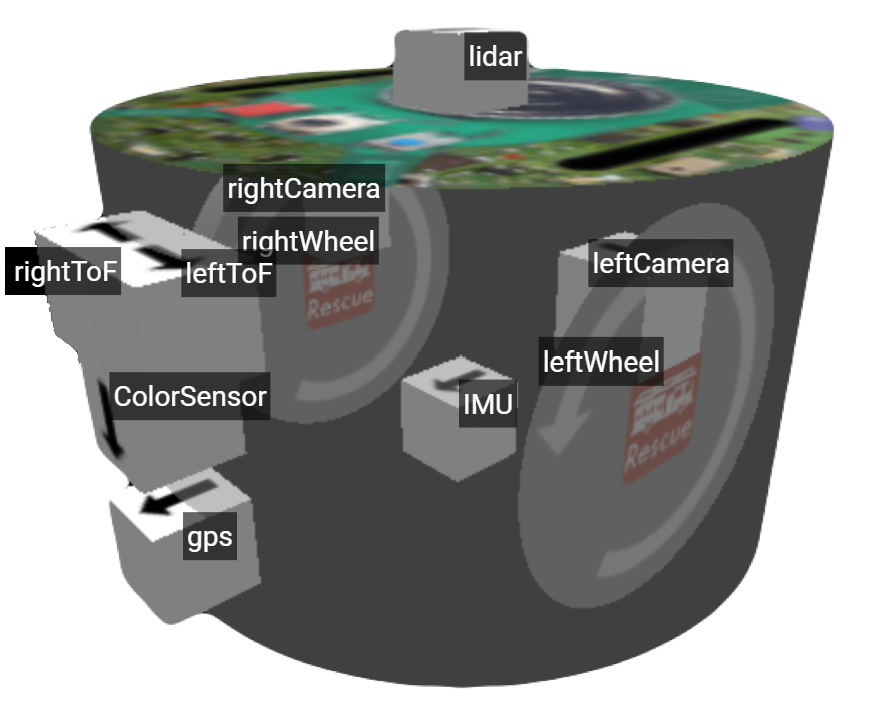
\includegraphics[width=70mm]{Photo/8107.PNG}
      
    \begin{itemize}
      \item 左右モータ+エンコーダ\\標準のものをそのまま使用している。
      \item IMU\\角度を取得するために使用している。
      \item GPS\\位置情報を取得するために使用している。
      \item カラーセンサ\\床の色情報を取得するために使用している。床との距離を近づけすぎないことで、チェックポイントタイルと通常タイルの判別をしやすくしている。
      \item 距離センサ\\くっついているだけの飾りである。いつか取ろうと思っていつまでたっても取っていない。
      \item LiDAR\\障害物の検知、壁の認識に使用している。
      \item 左右カメラ\\被災者の検知に使用している。
    \end{itemize}
  

  \section{使用しているプログラミング言語・ソフトウェア}
  \noindent
  主な開発環境
  \begin{itemize}
    \item Webots 2023.a
    \item Erebus v23.0.5
    \item C++ 14 (メイン言語)
    \item Python 3.12.1
    \item Visual Studio 2022
  \end{itemize}

  使用した言語はC++である。殊レスキューシミュレーションにおいてはPythonの方がポピュラーであることは何となしに知っていたが、C++の方が好みなのでC++を採用した。\\
  もちろん、画像認識の選択肢が狭まることは承知の上である。\\

  Visual Studioの環境構築には苦労した。なにせ、レスキューシミュレーション公式サイトにもDiscordにも情報がないのである。結果的には、Webotsの公式サイトの情報を基に作成した。このままではよくないと思い、簡単にだが環境構築方法をまとめたページを作成した。\url{https://qiita.com/kikou0517/items/f13045b6b97767e7d0f0}\\
  
  \noindent
  使用ライブラリ
  \begin{itemize}
    \item OpenCV 4.8.0
  \end{itemize}

  \section{被災者・ハザードマップ}
  考えたくない泣

  \section{探索アルゴリズム}
  深さ優先探索を使用する。探索は6cm単位で行う。\\
  オリジナルの工夫点も加えた。\\
  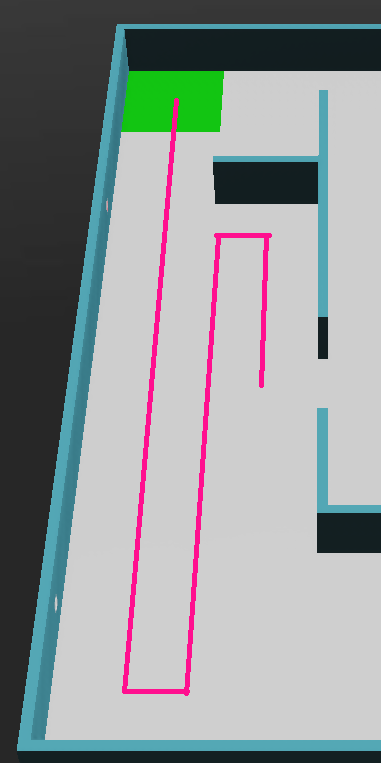
\includegraphics[width=40mm]{Photo/feagure1.png}

  上図のマップでは、ピンク線で示したように探索済みのマスを半分跨ぎながら進むという効率の悪い探索を行う可能性がある。これは機体のサイズは12$\times$12cmを基準とするのに対して、6cm単位で探索を行うことが原因である。\\
  そこで深さ優先探索における「未探索」「探索済み」という2つのパラメーターに「部分的に探索済み」を加え、進行方向の候補が複数あった場合に「部分的に探索済み」の優先度を下げることで、上図のような探索を防いでいる。\\

  \section{アピールポイント}
    \subsection{情報公開}
    情報公開はロボカップジュニアの国是のようなものである。\\
    シミュレーションリーグでコードをオープンにすることは、実機リーグのそれとは持つ意味合いが少し違うと思っている。良くも悪くも、たった1つのexeファイルが文字通り「全て」なのだから。だが、RCJJのコミュニティに何か少しでも貢献できることがあればと思い、今年もソースコードを大会終了後に公開することにした。\\
    実際にこのソースコードを公開することで直接誰かの参考になるとはあまり思っていない。それよりも、自分を含めより多くの人が情報公開をすることで、よりコミュニティが活発になることに期待して公開を決めた。\\
    また、公開することで、自分自身の成長を促すことにもなる。自分のコードを他人に見せることで、自分のコードに対する意識が変わる。\\

    去年のリポジトリも公開状態だが、ポスターに明記していなかったため、アクセスする方法が限られていた。今年はポスターに載せているのでそのようなことにはならないはずである。\\
    

    \subsection{アソビゴコロ}
    ずっとカラフルな文字と黒い背景ににらめっこしていると、目だけじゃなくて心まで疲れてくる。\\
    そこでちょっとした遊び心を取り入れてみた。\\
    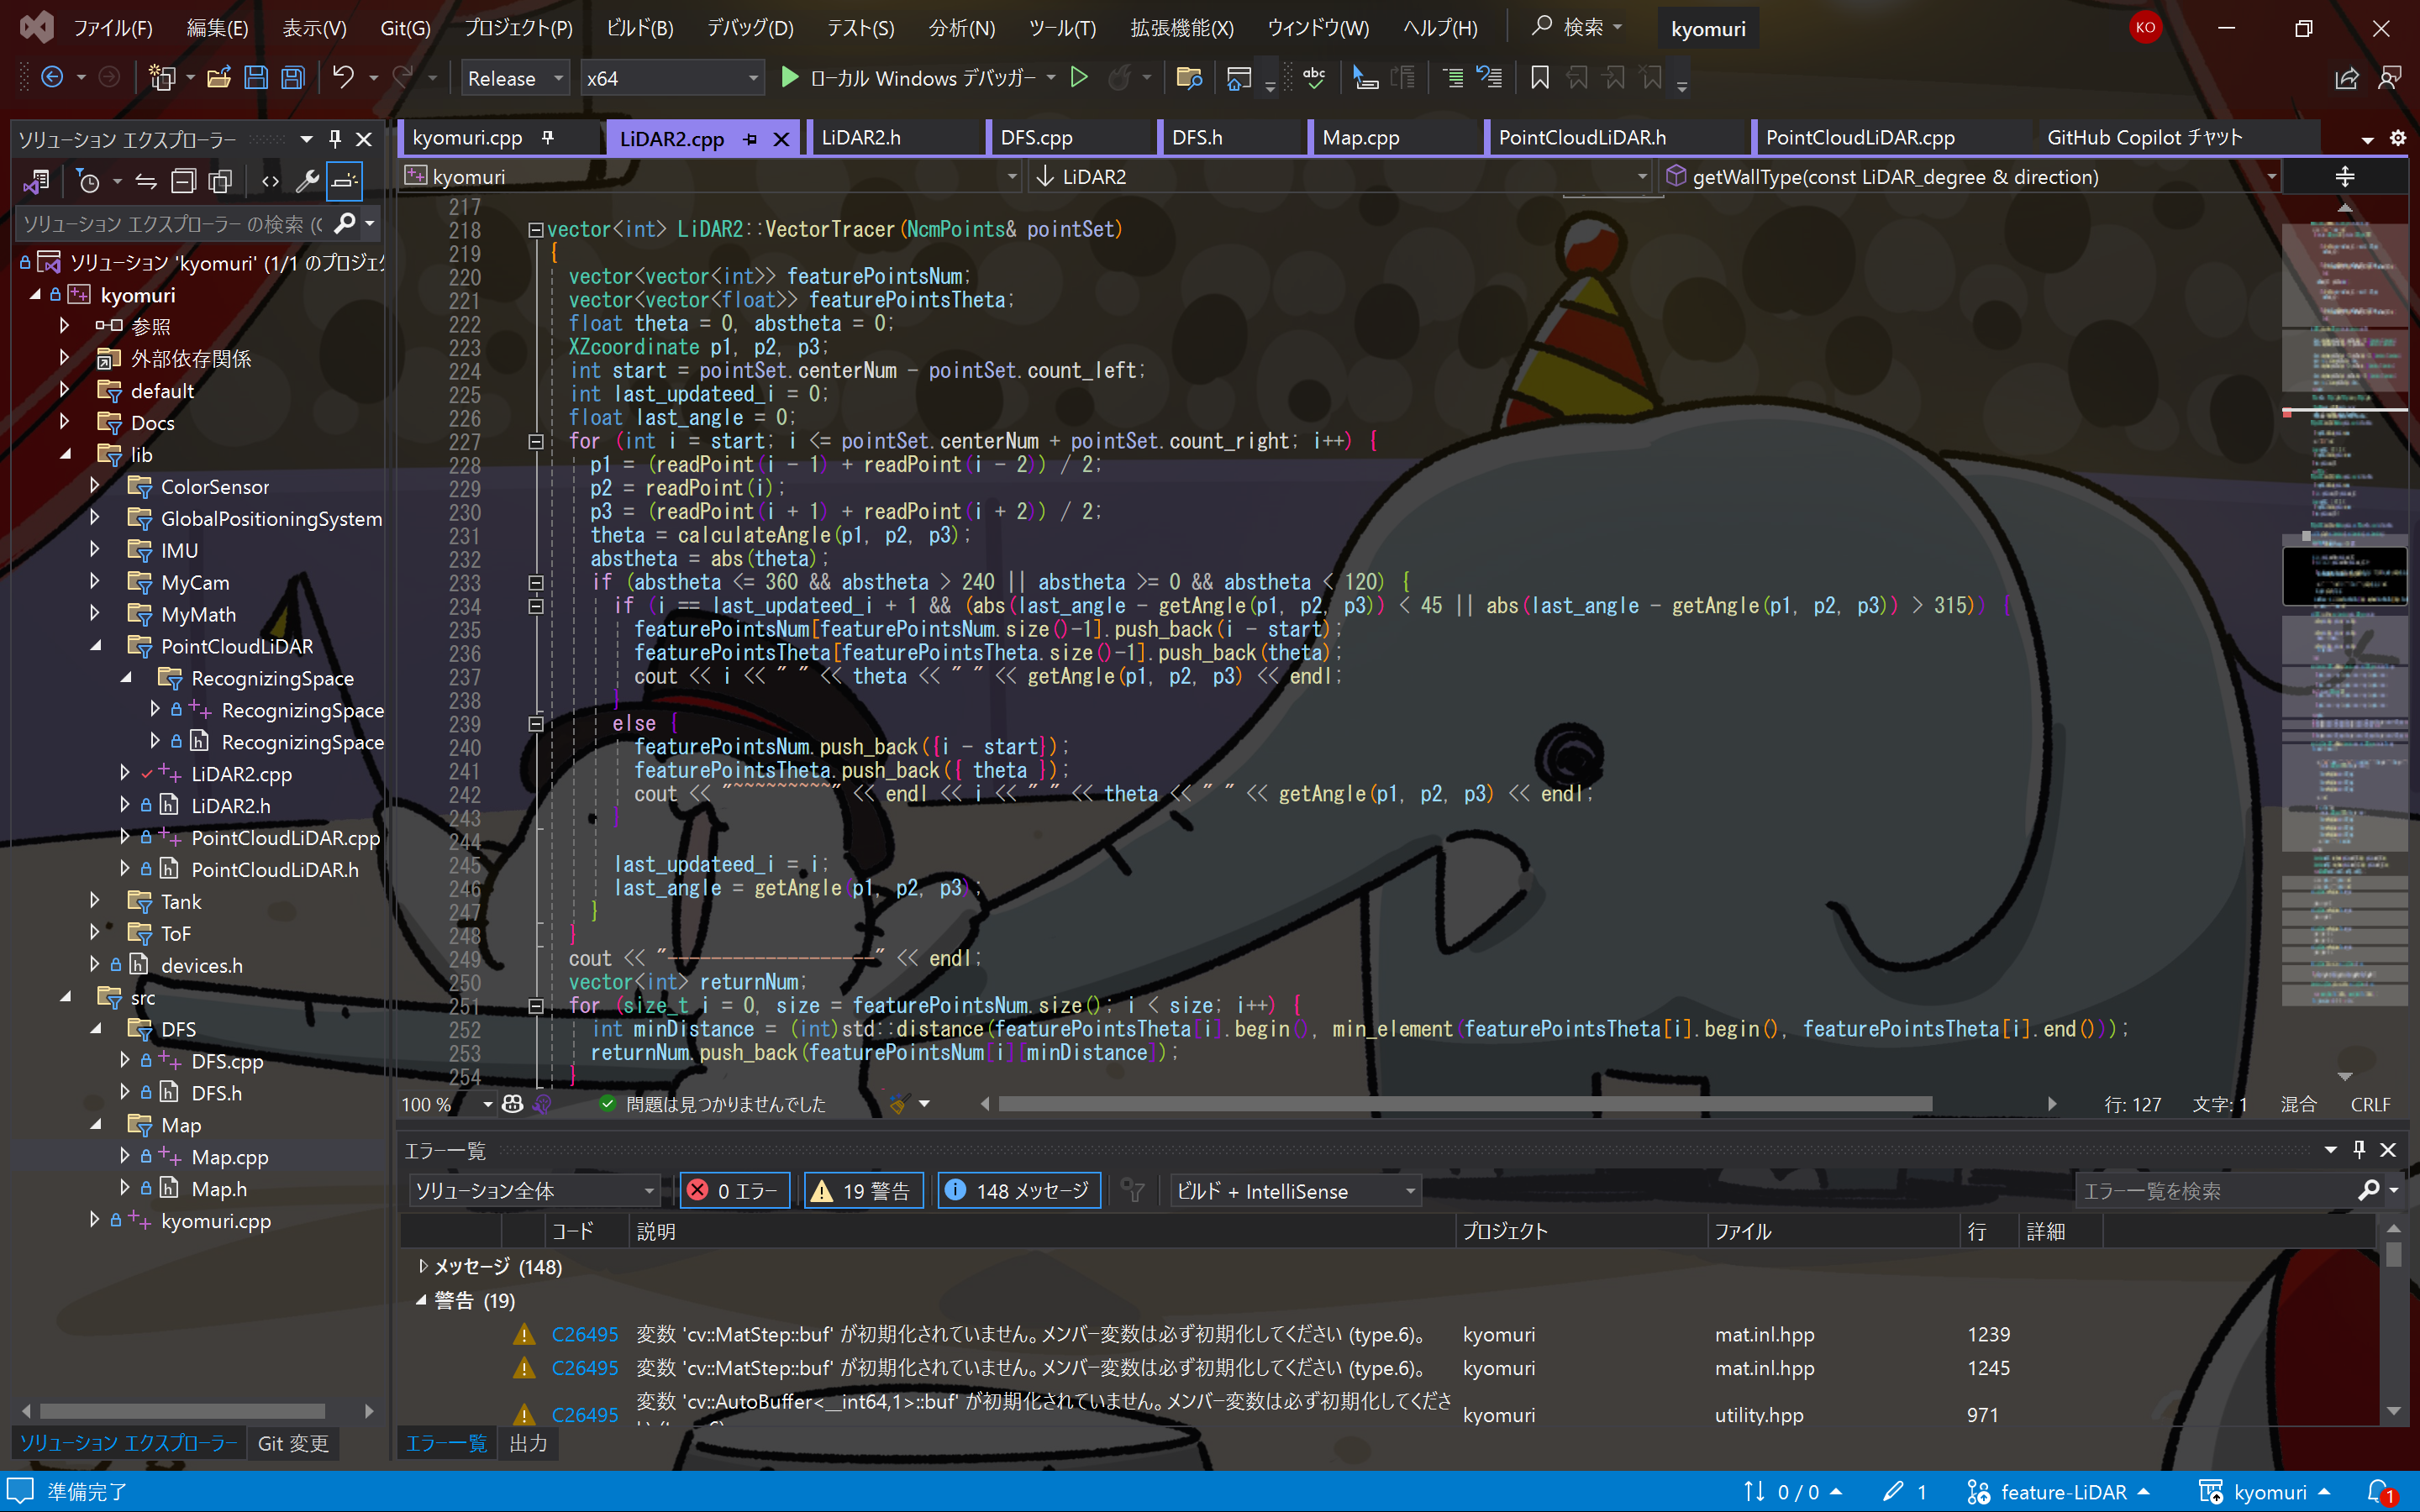
\includegraphics[width=100mm]{Photo/photo0.png}\\
    Visual Studioの画面である。見ての通り、背景にキャラクターの画像を設定している。\\

    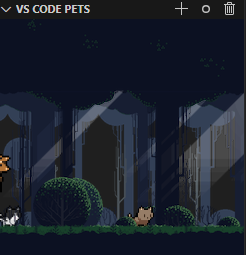
\includegraphics[width=50mm]{Photo/photo2.png}\\
    Viaual Studio Codeではvscode-petsという拡張機能を使用して、いつでも猫を眺めることができる。\\

    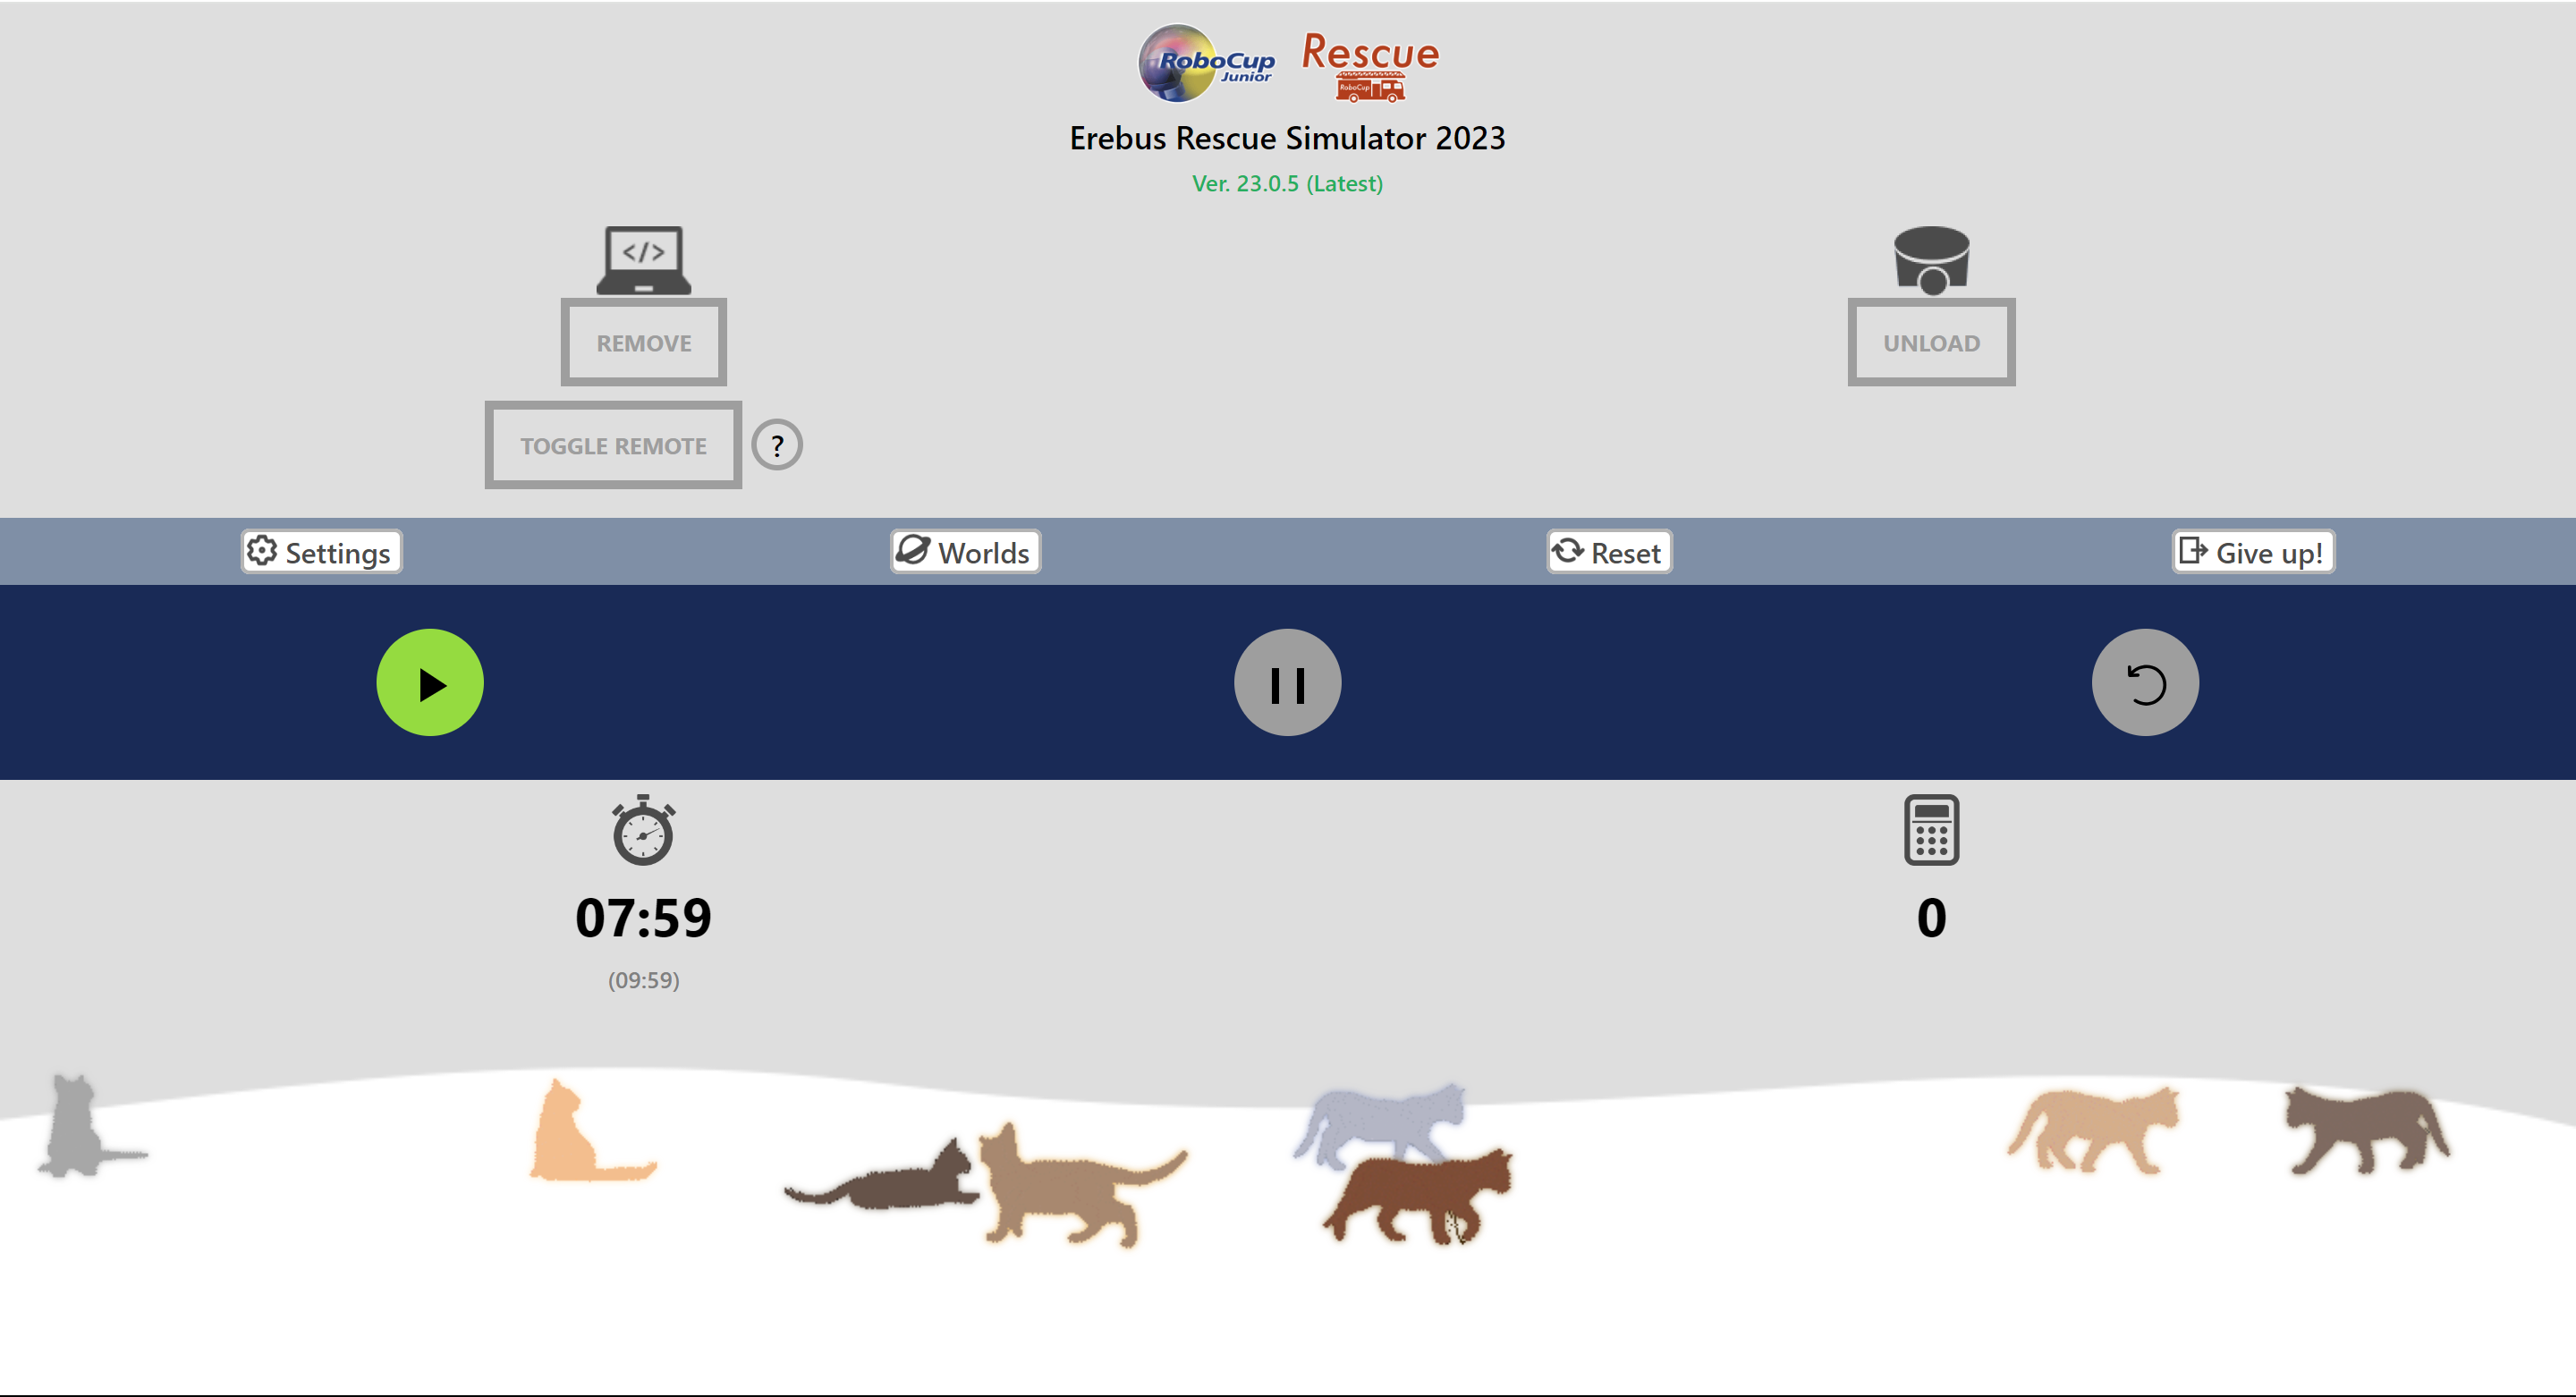
\includegraphics[width=100mm]{Photo/photo3.png}\\
    ブラウザを開けば、やはり猫がいる。"ネッコサーフィン"という拡張機能だ。\\

    こうやって、たまに癒されいている。\\


\end{document}